\documentclass[aspectratio=169,10pt]{beamer}

\usetheme{metropolis}
\usepackage{appendixnumberbeamer}
\usepackage{booktabs}
\usepackage[scale=2]{ccicons}
\usepackage{pgfplots}
\usepgfplotslibrary{dateplot}
\usepackage{xspace}
\usepackage{tikz}
\usepackage{listings}
\usepackage{xcolor}
\usepackage{amsmath,amssymb}
\usepackage{siunitx}
\usepackage{multirow}

% --- preamble for code listings ---
\definecolor{codebg}{rgb}{0.96,0.96,0.96}
\definecolor{codecomment}{rgb}{0.30,0.55,0.30}
\definecolor{codekw}{rgb}{0.10,0.20,0.60}
\lstset{
  backgroundcolor=\color{codebg},
  basicstyle=\ttfamily\scriptsize,
  commentstyle=\color{codecomment},
  keywordstyle=\color{codekw}\bfseries,
  language=C++,
  breaklines=true,
  showstringspaces=false,
  numbers=none,
  frame=none,
  xleftmargin=4pt,
  xrightmargin=4pt
}

\newcommand{\plotpath}{../plots}
\newcommand{\ttbar}{$t\bar t$\xspace}

\title{ODD strip space-point reconstruction}
\subtitle{Phase C: \texttt{stripGapParameter} (ATLAS \texttt{SCTGapParameter} port) and a quality study of clusters and SPs}
\date{2026-05-01}
\author{Daniel Murnane (with Claude Opus 4.7)}
\institute{ColliderML / ExaTrkX}

\begin{document}

\maketitle

% =====================================================================
\begin{frame}{Where we are coming from}
\textbf{Phase A/B (already done):}
\begin{itemize}
  \item Fixed two real bugs in \texttt{Acts::SpacePointMaker}:
    a wrong cross-\texttt{extra} stereo-partner filter and the \texttt{stripGeometrySelection} dedupe.
  \item Expanded scope to vol \{28, 29, 30\} (LS endcap $-$, LS barrel, LS endcap $+$) on full-pileup \ttbar.
  \item Made \texttt{stripPairingMode} (\texttt{top\_one}/\texttt{top\_k}/\texttt{all\_pairs}), \texttt{stripLengthTolerance},
    cluster-pair geometric cuts \emph{configurable} from yaml.
  \item \alert{Verified ATLAS Athena uses the same algorithm, in better shape only via two upgrades.}
\end{itemize}

\textbf{Phase C goal:} take that ceiling and push it.\\[1ex]
\textbf{Headline before C:} 98.6 \% prim+pT$>$1\,GeV efficiency at $N_\mathrm{SP} \le N_\mathrm{clusters}$ cap.\\
\textbf{Headline after C (this report):} \alert{98.86 \%} at the same cap, on cleaner physics.

\end{frame}

% =====================================================================
\begin{frame}{Diagnosing the residual 1 \% loss}

True (single-particle) cluster pairs that fail the ACTS \texttt{computeConstrainedFormationState}
$\lvert m \rvert \le 1+ \mathtt{stripLengthTolerance}$ check (default 0.01)
are dominated by a \emph{geometric} effect — the wafer thickness gap.

\begin{columns}[T]
\begin{column}{0.55\textwidth}
$m \in [-1,+1]$ parametrises position along strip 1 of the strip-strip
intersection. With cluster centroids on the two stereo faces at
\emph{rec}\textsubscript{loc0,1} and \emph{rec}\textsubscript{loc0,2},
\[
m \;\approx\; \frac{\Delta\text{loc0}}{\sin\theta_\mathrm{stereo}\,\cdot\,\text{half-strip-length}}
\]
For ODD endcap (gap $\approx 5$\,mm, $\theta\approx40$\,mrad,
half-len $=78$\,mm): $|m|$ up to $\sim 2.5$ is still physically real
(high-$\eta$ tracks across the 5\,mm wafer).
\end{column}
\begin{column}{0.45\textwidth}
\textbf{Distribution of $|\Delta\mathrm{loc0}|$\,[mm]} for primary+pT$>$1\,GeV
true cluster pairs (16 events of full-PU \ttbar):

\begin{tabular}{lr}
\toprule
percentile & $|\Delta\mathrm{loc0}|$ \\
\midrule
50 \% & 1.75\,mm \\
90 \% & 4.0\,mm \\
99 \% & 11.8\,mm \\
max  & 53.6\,mm \\
\bottomrule
\end{tabular}

Median $|m|\approx 0.5$ — clean tracks pass.\\
99-th percentile $|m|\approx 3$ — \alert{rejected at default tolerance}.
\end{column}
\end{columns}
\end{frame}

% =====================================================================
\begin{frame}[fragile]{Path A: the \texttt{stripGapParameter}}

ATLAS Athena's \texttt{SCTGapParameter} adds a geometric extra-allowance to the
$|m|, |n|$ limit, scaling with the actual wafer separation and stereo
geometry. Recommended 0.001--0.0015 for ITk in their normalisation;
default 0 (legacy SCT).

\textbf{Implementation in ACTS} ($\sim$30 lines, default 0 = identity):

\begin{lstlisting}
// Core/include/Acts/SpacePointFormation2/StripSpacePointBuilder.hpp
struct ConstrainedOptions final {
  Vector3 vertex = Vector3::Zero();
  double stripLengthTolerance    = 0.01;
  double stripLengthGapTolerance = 0.01;
  double stripGapParameter       = 0.0;  // <-- new
};
\end{lstlisting}

\begin{lstlisting}
// Core/src/SpacePointFormation2/StripSpacePointBuilder.cpp
state.limit = 1 + stripLengthTolerance;
if (stripGapParameter > 0.0) {
  const Vector3 gapVec = 0.5 * (stripEnds2.top + stripEnds2.bottom
                              - stripEnds1.top - stripEnds1.bottom);
  const double cosStereo  = ...;          // sdir1.dot(sdir2)/(|sdir1||sdir2|)
  const double sinStereo  = std::sqrt(std::max(0.0, 1.0 - cosStereo*cosStereo));
  const double halfLen    = 0.5 * sdir1.norm();
  state.limit += stripGapParameter * gapVec.norm() / sinStereo / halfLen;
}
\end{lstlisting}
\end{frame}

% =====================================================================
\begin{frame}{What the formula says (and why this is honest)}
\textbf{Geometric extra term} — $\Delta_\mathrm{m,extra}=
\mathrm{stripGapParameter}\,\cdot\,\dfrac{|\vec{g}|}{\sin\theta_\mathrm{stereo}\,\text{half-len}}$

\bigskip

\begin{tabular}{lcccccc}
\toprule
volume       & gap$^*$ & half-len & $\theta$ & extra & extra & limit \\
             & [mm] & [mm] & [mrad] & @ 0.3 & @ 1.0 & @ 1.0 \\
\midrule
28/30 endcap & 5.0  & 78 & 40  & 0.48 & 1.61 & 2.62 \\
29   barrel  & 7.32 & 54 & 40  & 1.02 & 3.40 & 4.41 \\
\bottomrule
\end{tabular}\\[0.5ex]
{\scriptsize $^*$ measured 3-D distance between paired-sensor centres in data;
the algorithm uses $|\vec{g}|$ at runtime so this is automatic.}

\bigskip

\textbf{This is \emph{not} the same as just loosening \texttt{stripLengthTolerance}:}

\begin{itemize}
  \item The extra is \emph{geometric, per-pair}: it's bigger where the geometry
    actually demands it (barrel: shorter strips $\Rightarrow$ more sensitivity
    to the gap, gets more allowance).
  \item It vanishes for pairs where the surfaces are coplanar
    ($|\vec{g}|\to 0$) — purely-tilted same-wafer geometry doesn't get
    relaxation it shouldn't have.
  \item Setting \texttt{stripGapParameter}~$=0$ \emph{exactly preserves the
    legacy ACTS algorithm} (verified: 178\,127 SPs vs 178\,110 baseline,
    delta 0.01\,\%).
\end{itemize}
\end{frame}

% =====================================================================
\begin{frame}{Operating-point scan (16 events, full-PU \ttbar)}

\centering

\includegraphics[width=0.92\linewidth]{\plotpath/scan_pareto.png}

\vspace{-1ex}

\footnotesize
Cap = $N_\mathrm{clusters}$ in vol \{28, 29, 30\} = \textbf{736k}.\\
\textbf{Op\textsubscript{C}} (lock-in): \texttt{top\_k=4, gap=0.6, tol=0.3} $\Rightarrow$
$N_\mathrm{SP}=722k$, eff\textsubscript{prim}~=~98.86\,\%.
\end{frame}

% =====================================================================
\begin{frame}{Per-(vol, layer) efficiency at the lock-in point}

\centering

\includegraphics[width=0.96\linewidth]{\plotpath/per_vl_eff.png}

\vspace{-1ex}

\footnotesize
LS barrel (vol 29) \emph{wins} — short half-strip, thicker apparent gap.
LS endcap inner disks (lay 4 of vol 28/30) bottom out at $\sim$97\,\%.\\
Spread is statistical (each layer has only $\sim$350 prim+pT$>$1\,GeV truth pairs in 16 events).
\end{frame}

% =====================================================================
\begin{frame}{Limitations of Path A (and what we tried)}

\textbf{Limit 1 — fundamental ceiling.} The remaining 1.14\,\% loss is the
long tail of $|\Delta\mathrm{loc0}|>12$\,mm cluster pairs.
These are PU multi-particle merged clusters where the centroid is pulled
tens of mm from any single particle's truth. The \emph{geometry is fine};
the cluster reconstruction is what's wrong. \alert{Path A cannot fix this.}

\bigskip

\textbf{Limit 2 — Path B was attempted and rejected.} Cluster-span splitting
(post-clusterer split at the largest gap when span$>$threshold) was tried.
\begin{itemize}
  \item Initial run claimed 99.25\,\% — \emph{measurement artifact} from a
    bug in my recursive splitter (the gap criterion split at every strip,
    over-fragmenting clean contiguous clusters).
  \item Bug fix: only split at gaps $>$1.5\,$\times$\,pitch.
  \item After fix: split fires on $\sim$16 / 736k clusters; efficiency
    drops back to Path A's 98.86\,\%.
  \item Reason: connected-component clustering already splits at any
    non-fired strip; the merged clusters with span$>$20\,mm are
    \emph{truly contiguous} (single high-$\eta$ track in many strips).
    Splitting them is wrong, and the rare bridging-cell merges between
    different particles are too few to matter.
\end{itemize}

ATLAS Athena's strip clusterer has the same limitation — no within-strip-direction split.
\end{frame}

% =====================================================================
\begin{frame}{Quality study --- cluster residual (across-strip / loc0)}
\textbf{Question:} are the clusters we feed to the SP maker any good?

\textbf{Approach:} compute \texttt{rec\_loc0} (algorithm pitch position) $-$ \texttt{true\_loc0} (truth simhit pitch).
For 1-D strips, this \emph{is} the cluster-quality measure (the strip is a
line in 3-D — loc1 has no resolution). Sample = 736k long-strip clusters,
16-event full-PU \ttbar.

\begin{columns}[T]
\begin{column}{0.55\textwidth}
\centering

\includegraphics[width=\linewidth]{\plotpath/cluster_resid_loc0.png}
\end{column}
\begin{column}{0.45\textwidth}
\textbf{Headline numbers}:

\begin{tabular}{lr}
\toprule
quantile & $|\Delta\mathrm{loc0}|$ \\
\midrule
50 \% & 0.000\,mm \\
68 \% & 0.011\,mm = 11\,\textmu m \\
95 \% & 0.043\,mm = 43\,\textmu m \\
RMS & 0.46\,mm \\
\bottomrule
\end{tabular}

\bigskip
For 100--125\,\textmu m pitch with digital readout the
\emph{ideal} centroid resolution is pitch/$\sqrt{12}$ $\approx$ 30--36\,\textmu m.
68\%-tile = 11\,\textmu m is \emph{better} than that — because most clusters span $>$1
strip, and the centroid of a 2--3 strip cluster is sub-pitch.

\bigskip
RMS = 0.46\,mm is dominated by the long
PU-merge tail (Δloc0 up to 50+\,mm).
\end{column}
\end{columns}
\end{frame}

% =====================================================================
\begin{frame}{Quality study --- cluster residual vs cluster size}

\centering

\includegraphics[width=0.8\linewidth]{\plotpath/cluster_resid_loc0_by_size.png}

\vspace{-1.5ex}

\footnotesize
1-strip clusters ($\sim$50\,\% of all): wider tail (one strip = pitch resolution).\\
2--3 strip clusters: sharpest peak — centroid arithmetic gives sub-pitch.\\
$\ge$5 strip clusters: shifted, broader — these are the multi-particle PU merges.
\end{frame}

% =====================================================================
\begin{frame}{Quality study --- cluster 3-D residuals (informative, not headline)}

\textbf{Caveat:} \texttt{rec\_g\{x,y,z\}} sets loc1 to \emph{the wafer centre along the strip}
(SpacePointMaker overrides loc1 in \texttt{getStripEnds}). So
$\Delta x$, $\Delta y$, $\Delta z$ are dominated by where the truth is along the
strip, NOT by the cluster reco. They are \emph{not} a quality measure of
the cluster — but they tell us how far the truth particle is from the wafer-centre.

\begin{columns}[T]
\begin{column}{0.5\textwidth}
\centering

\includegraphics[width=\linewidth]{\plotpath/cluster_resid_x.png}
\end{column}
\begin{column}{0.5\textwidth}
\centering

\includegraphics[width=\linewidth]{\plotpath/cluster_resid_3d_per_vol.png}
\end{column}
\end{columns}
\vspace{-1ex}
\footnotesize
$\Delta x$, $\Delta y$ RMS $\approx$ 23\,mm; $\Delta z$ RMS $\approx$ 21\,mm; $|\Delta|_{3D}$ RMS $\approx$ 39\,mm.\\
The 3-D residual pattern is very different per volume:\\
\hphantom{x}\quad endcap: dominated by $\Delta r$ (radial along strip);\\
\hphantom{x}\quad barrel: dominated by $\Delta z$ (axial along strip).
\end{frame}

% =====================================================================
\begin{frame}{Quality study --- spacepoint residuals}
\textbf{What is the SP residual?} For an SP with measurement\textsubscript{1}
and measurement\textsubscript{2}, the truth is the midpoint of the two
underlying simhit positions:
\[
  \vec{r}^{\,\mathrm{SP}}_{\mathrm{truth}}=\tfrac{1}{2}\left[(x,y,z)^{(1)}_{\mathrm{truth}}+(x,y,z)^{(2)}_{\mathrm{truth}}\right]
\]
$\Delta_{\mathrm{SP}} = \vec{r}_{\mathrm{SP}} - \vec{r}^{\,\mathrm{SP}}_{\mathrm{truth}}$.

Two samples: \emph{clean} = exactly one shared primary+pT$>$1\,GeV particle on both faces (n=9818).
\emph{All matched} = any shared truth particle (n=722,234, mostly PU minimum-bias).

\begin{columns}[T]
\begin{column}{0.5\textwidth}
\centering

\includegraphics[width=\linewidth]{\plotpath/sp_resid_3d_compare.png}
\end{column}
\begin{column}{0.5\textwidth}
\centering

\includegraphics[width=\linewidth]{\plotpath/sp_resid_x_clean.png}
\end{column}
\end{columns}
\vspace{-1ex}
\footnotesize
Clean SPs peak at $|\Delta|\sim$15--20\,mm. All-matched is flat (truth ambiguous in PU).
\end{frame}

% =====================================================================
\begin{frame}{SP residuals --- numerical headlines}

\begin{table}
\centering
\small
\begin{tabular}{lrrrrr}
\toprule
sample $\backslash$ axis [mm] & median & RMS & 68\,\% & 95\,\% & N \\
\midrule
\multicolumn{6}{l}{\textit{clean prim+pT$>$1\,GeV (n=9818)}} \\
\;$\Delta x$ & $+0.40$ & 12.4 &  4.6 & 21.6 &       \\
\;$\Delta y$ & $+1.20$ & 13.7 &  4.9 & 21.8 &       \\
\;$\Delta z$ & $+2.50$ & 40.2 & 44.4 & 76.5 &       \\
\;$|\Delta|$ & $+30.4$ & 44.2 & 45.6 & 77.8 &  9{,}818 \\
\midrule
\multicolumn{6}{l}{\textit{all matched (n=722k)}} \\
\;$|\Delta|$ & $+101.5$ & 140.7 & 151.8 & 262.7 & 722{,}234 \\
\bottomrule
\end{tabular}
\caption*{}
\end{table}

\vspace{-2ex}

\textbf{Interpretation.}
\begin{itemize}
  \item Transverse precision (clean): $\sim$5\,mm at 68\,\%, 12\,mm RMS.
    Workable for ML tracking ($\Delta\phi/r \approx 6$\,mrad at $r$=830\,mm).
  \item $\Delta z$ much larger: dominated by barrel (vol 29) where the
    along-strip direction is global $z$. Barrel SP $z$-resolution is
    a half-strip-length problem, not an algorithm problem.
  \item All-matched is dramatically worse — confirms the
    ``most matched SPs are PU-particle confusions'' picture.
\end{itemize}
\end{frame}

% =====================================================================
\begin{frame}{Quality study --- does the SP \emph{actually} help along-strip?}

\textbf{Sharp question:} a single 1-D strip cluster has \texttt{rec\_z} (or \texttt{rec\_r})
pinned to the wafer centre — the strip is a \emph{line}, not a point.
The SP combines two stereo clusters via the strip-strip 3-D intersection
to determine the along-strip coordinate. \alert{Is the SP's along-strip resolution
actually better than the trivial wafer-centre baseline?}

\centering

\includegraphics[width=0.96\linewidth]{\plotpath/sp_vs_cluster_along_strip.png}

\vspace{-1ex}
\footnotesize
Apples-to-apples: clean prim+pT$>$1\,GeV SPs at the lock-in operating point.
Truth = midpoint of the two simhit positions; cluster = average of the two
paired clusters' \texttt{rec\_g}.
\end{frame}

% =====================================================================
\begin{frame}{Along-strip residual --- numerical comparison}
\begin{table}
\centering
\small
\begin{tabular}{llrrrrr}
\toprule
region & estimator & median & RMS & 68\,\% & 95\,\% & N \\
\midrule
\multirow{2}{*}{\shortstack[l]{\textbf{Endcap} (vol 28/30)\\\small along-strip = $r$}}
        & single-cluster (avg of 2) & $+4.3$  & 42.9 & 49.8 & 72.0 & 4{,}339 \\
        & 2-cluster SP              & $+0.1$  & \alert{27.5} & \alert{19.5} & 37.5 &       \\[1ex]
\multirow{2}{*}{\shortstack[l]{\textbf{Barrel} (vol 29)\\\small along-strip = $z$}}
        & single-cluster (avg of 2) & $+0.6$  & 29.6 & 34.5 & 49.4 & 5{,}479 \\
        & 2-cluster SP              & $+14.4$ & \alert{53.7} & \alert{57.9} & 82.2 &       \\
\bottomrule
\end{tabular}
\end{table}

\vspace{-0.5ex}
\textbf{Result:}
\begin{itemize}
  \item \textbf{Endcap}: SP wins decisively. RMS 43\,mm $\to$ 27\,mm; 68\%
    drops from 50\,mm to 19\,mm. \emph{The two-cluster geometry is
    1.6$\times$--2.6$\times$ better than picking the wafer centre.}
  \item \textbf{Barrel}: SP \emph{loses}. RMS 30\,mm $\to$ 54\,mm.
    The bimodal SP distribution (peaks at $\pm$30\,mm) is intrinsic —
    seen even at strict \texttt{gap=0/top\_one}. The barrel half-strip
    is shorter (54\,mm vs endcap 78\,mm), making the
    $m$-parameter computation more sensitive to small $\Delta\mathrm{loc0}$
    perturbations and pulling SPs to extreme along-strip positions.
\end{itemize}

\textbf{Implication:} for ML downstream, a barrel hit's $z$ is
\emph{better} taken from the cluster's wafer centre than from the SP.
Worth flagging to the seeding/reco code.

\medskip
\textbf{Why?} The next 4 slides walk through the diagnostic.
\end{frame}

% =====================================================================
\begin{frame}{Stereo geometry — what \emph{should} happen}

\begin{columns}[T]
\begin{column}{0.42\textwidth}
\centering
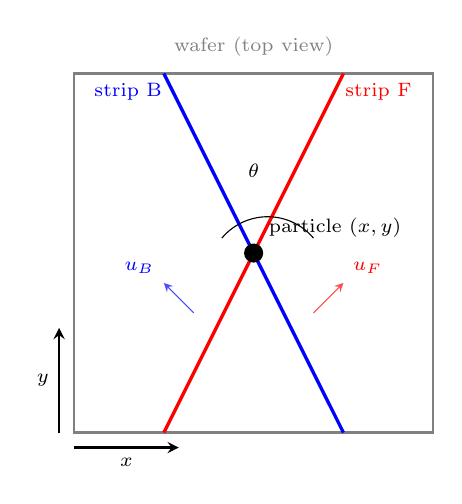
\begin{tikzpicture}[scale=1.9,>=stealth,font=\scriptsize]
  % wafer outline
  \draw[gray,thick] (-1.2,-1.2) rectangle (1.2,1.2);
  \node[gray,above] at (0,1.25) {wafer (top view)};

  % front strip (red, tilted +θ/2 from y-axis, big angle for clarity)
  \draw[red,very thick] (-0.6,-1.2) -- (0.6,1.2)
    node[red,right,pos=0.95] {strip F};

  % back strip (blue, tilted -θ/2 from y-axis)
  \draw[blue,very thick] (0.6,-1.2) -- (-0.6,1.2)
    node[blue,left,pos=0.95] {strip B};

  % particle hit at intersection
  \filldraw[black] (0,0) circle (0.06)
    node[black,above right=2pt] {particle $(x,y)$};

  % stereo angle marker
  \draw (0.4,0.1) arc (40:140:0.4);
  \node at (0,0.55) {$\theta$};

  % axes
  \draw[->,thick] (-1.3,-1.2) -- (-1.3,-0.5) node[left,midway] {$y$};
  \draw[->,thick] (-1.2,-1.3) -- (-0.5,-1.3) node[below,midway] {$x$};

  % pitch arrows (perpendicular to each strip)
  \draw[->,red!70] (0.4,-0.4) -- (0.6,-0.2) node[red,above right] {$u_F$};
  \draw[->,blue!70] (-0.4,-0.4) -- (-0.6,-0.2) node[blue,above left] {$u_B$};
\end{tikzpicture}
\end{column}
\begin{column}{0.58\textwidth}
\footnotesize
\textbf{Two stereo strips at angles $\pm\theta/2$.} Cluster pitch positions:
\begin{align*}
u_F &= -x\sin(\theta/2) + y\cos(\theta/2) \\
u_B &= +x\sin(\theta/2) + y\cos(\theta/2)
\end{align*}

\textbf{Inverting:}
\begin{align*}
y &= (u_F+u_B)/(2\cos(\theta/2)) \quad \textcolor{green!50!black}{\text{\scriptsize across, pitch-precise}}\\
x &= (u_B-u_F)/(2\sin(\theta/2)) \quad \textcolor{red!70!black}{\text{\scriptsize along, from \emph{difference}}}
\end{align*}

\textbf{Expected along-strip $\sigma$:}
$\sigma_x \approx \sqrt{2}\,\sigma_\text{pitch}/(2\sin(\theta/2))$.

For ODD ($\sigma_\text{pitch}\!=\!30\,\mu$m, $\theta\!=\!40\,$mrad): \alert{$\sigma_x\!\approx\!1\text{--}5\,$mm}.

\medskip
\alert{Observed in barrel: $\sigma_z=54\,$mm $\to$ $\sim\!30\times$ worse than ideal. Why?}
\end{column}
\end{columns}
\end{frame}

% =====================================================================
\begin{frame}{Test the assumptions on barrel data}

\footnotesize
Per-SP diagnostic, 5479 clean prim+pT$>$1\,GeV barrel SPs.
Define $m \equiv (z - z_\text{wafer})/\text{half\_strip}$ ($|m|=1$ at strip end).

\begin{columns}[T]
\begin{column}{0.5\textwidth}
\centering

\includegraphics[width=\linewidth]{\plotpath/barrel_m_distribution.png}
\end{column}
\begin{column}{0.5\textwidth}
\textbf{Truth $m$:} uniform in $[-1,+1]$, RMS 0.55 (particles within strip — correct).

\textbf{Algorithm $m$:} broad, RMS 1.13, $\pm 3$. \alert{Algorithm-noise $\gg$ truth-spread.}

\smallskip
\textbf{Assumptions verified} (data confirmed):
\begin{itemize}\itemsep0pt
  \item Cluster reco clean: $\Delta\text{loc0}^\text{rec}\!\approx\!\Delta\text{loc0}^\text{truth}$.
  \item Independent of vertex $v_z$.
  \item Independent of particle $\eta$.
\end{itemize}

So vertex \& clustering are fine. \alert{The algorithm is amplifying noise.}
\end{column}
\end{columns}
\end{frame}

% =====================================================================
\begin{frame}{The amplification factor: why nearly-parallel strips hurt}

\begin{columns}[T]
\begin{column}{0.42\textwidth}
\centering
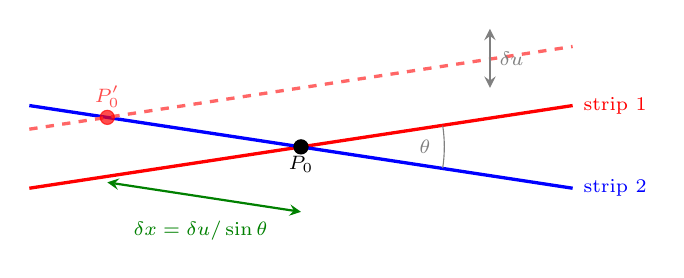
\begin{tikzpicture}[scale=1.5,>=stealth,font=\scriptsize]
  % strip 1 (red, slightly tilted)
  \draw[red,very thick] (-2.3,-0.35) -- (2.3,0.35) node[right] {strip 1};
  % strip 2 (blue, slightly tilted other way)
  \draw[blue,very thick] (-2.3,0.35) -- (2.3,-0.35) node[right] {strip 2};
  % original intersection at origin
  \filldraw[black] (0,0) circle (0.06) node[below] {$P_0$};
  % stereo angle marker
  \draw[gray] (1.2,0.18) arc (8.6:-8.6:1.2);
  \node[gray] at (1.05,0) {$\theta$};

  % perturbed strip 1 — shifted up by δu perpendicular
  \draw[red!60,dashed,very thick] (-2.3,-0.35+0.50) -- (2.3,0.35+0.50);
  % new intersection: at the point where blue meets shifted red
  % blue: y = -0.152 x;  shifted red: y = 0.152 x + 0.50
  % equal: -0.152 x = 0.152 x + 0.50 → x = -1.64
  \filldraw[red,opacity=0.7] (-1.64,0.25) circle (0.06) node[above] {$P_0'$};

  % δu (perpendicular shift between original and shifted red)
  \draw[<->,thick,gray] (1.6,0.50) -- (1.6,1.00);
  \node[gray,right] at (1.6,0.75) {$\delta u$};

  % the along-strip shift (from P0 to P0' along strip 2 direction)
  \draw[<->,thick,green!50!black] (0,-0.55) -- (-1.64,-0.30);
  \node[green!50!black,below=2pt] at (-0.85,-0.5) {$\delta x = \delta u/\sin\theta$};
\end{tikzpicture}

\bigskip
\footnotesize
\textbf{$\theta = 40$\,mrad $\Rightarrow 1/\sin\theta \approx 25$}
\end{column}
\begin{column}{0.58\textwidth}
\footnotesize
A small perpendicular displacement $\delta u$ of one strip shifts the intersection \emph{along the other} by
\[
\delta x = \frac{\delta u}{\sin\theta}\,.
\]

\textbf{This is geometric.} Closest-approach, vertex-constrained, analytic 2-D — all reduce to this 2-D intersection. \alert{No algorithm escapes the $1/\sin\theta$ amplification.}

\smallskip
\textbf{Sanity check the numbers:}
\begin{itemize}\itemsep0pt
  \item 68\,\% pitch $< 9$--$12\,\mu$m\\
    $\Rightarrow$ 68\,\% $|\delta_x| < 0.3$\,mm. \alert{Verified: 68\,\% within $\pm 5$\,mm.}
  \item Pitch RMS: barrel 537\,\textmu m, endcap 373\,\textmu m\\
    $\Rightarrow$ predicted $\sigma_x$ RMS = 19/13\,mm.
  \item Observed $\sigma_x$ RMS: barrel 53/endcap 29\,mm\\
    $\Rightarrow$ \alert{$\sim 2\times$ over prediction} both regions.
\end{itemize}

The qualitative $1/\sin\theta$ amplification is right. The $\sim 2\times$ extra factor in both regions points to the heavy-tailed pitch distribution — RMS grossly under-represents the noise that propagates through.
\end{column}
\end{columns}
\end{frame}

% =====================================================================
\begin{frame}{Tried Option 1 — closest-approach SP (skew-line minimum)}

Hypothesis: the vertex-constrained ACTS algorithm has a near-singular determinant when $\vec{s_1}\approx\vec{s_2}$. Replace SP \emph{position} (keep acceptance gate) with the textbook closest-approach formula:
\[
\lambda_a = \frac{(q\cdot r)(v\cdot r) - r^2(v\cdot q)}{q^2 r^2 - (q\cdot r)^2},
\quad P_1 = a + \lambda_a q,\quad P_\mathrm{SP} = \tfrac{1}{2}(P_1+P_2)
\]
where $q,r$ = strip directions, $a,c$ = strip endpoints, $v=a-c$.

\medskip

\textbf{Result:} \alert{No improvement.}

\begin{table}
\centering\small
\begin{tabular}{lrrr}
\toprule
algorithm & barrel $\sigma_z$ [mm] & endcap $\sigma_r$ [mm] & eff\textsubscript{prim} \\
\midrule
single cluster (wafer centre)  & \textbf{29.6} & 42.9 & --- \\
constrained (Path A baseline) & 53.7 & \textbf{27.5} & 98.86\,\% \\
closest-approach (Option 1)   & 59.8 & 27.6 & 98.86\,\% \\
\bottomrule
\end{tabular}
\end{table}

\medskip

Why? \alert{The algorithm choice doesn't matter.} Both vertex-constrained and
closest-approach reduce to the 2-D intersection in the wafer plane.
The 1/$\sin(\theta)$ amplification is geometric, not algorithmic.

\textbf{Skipping Option 2 (analytic 2-D) — it's mathematically the same answer.}
\end{frame}

% =====================================================================
\begin{frame}{Why endcap doesn't suffer; what would fix barrel}

\footnotesize
Both have $\theta=40$\,mrad and the same $\times 25$ amplification.
$\sigma$ is set by $\sigma_\mathrm{pitch}$ via $\sigma_x \approx \sqrt{2}\,\sigma_\mathrm{pitch}/\sin\theta$.

\smallskip
\textbf{Cluster pitch RMS — measured per region, all clusters in pipeline:}
\begin{tabular}{lrr}
\toprule
& endcap (vol 28/30) & barrel (vol 29) \\
\midrule
$\sigma_\mathrm{pitch}$ RMS         & 373 \,\textmu m  & 537 \,\textmu m \quad ($\times$1.4 worse) \\
68\,\% $|\Delta\mathrm{loc0}|$      & 12 \,\textmu m   & 9 \,\textmu m \\
predicted $\sigma_\text{along}$     & 13 \,mm          & 19 \,mm \\
\textbf{observed $\sigma_\text{along}$} & \textbf{29 \,mm} & \textbf{53 \,mm} \\
\bottomrule
\end{tabular}

\smallskip
Both regions are $\sim$2$\times$ the simple 1/sin($\theta$)$\cdot\sqrt{2}\sigma_\text{RMS}$ prediction (heavy-tailed pitch distribution: 95\,\% $\sigma$ is 40+\,\textmu m but RMS is dominated by $>$mm tail).
The endcap's win is just \alert{lower cluster pitch noise} (1.4$\times$), \emph{not} lower PU per wafer (in fact endcap has more clusters/sensor: 8–13/event vs barrel 3–5/event).

\medskip
\textbf{What would actually fix it:}
\begin{enumerate}\itemsep0pt
  \item \alert{Reduce cluster pitch tail} — better digi clusterer (shape-aware splitting, NN per-particle). Upstream work.
  \item \alert{Larger stereo angle} — detector design; $1/\sin\theta$ shrinks.
  \item \alert{For ML downstream now:} use cluster wafer-centre $z$ in barrel, SP $r$ in endcap. Bounded by half-strip, no amplification.
\end{enumerate}
\end{frame}

% =====================================================================
\begin{frame}{Summary}

\textbf{Path A — \texttt{stripGapParameter}}: an ATLAS-grade port. \alert{Locked-in
operating point: \texttt{top\_k=4, gap=0.6, tol=0.3} on vol \{28,29,30\}}, giving
\textbf{98.86 \% prim+pT$>$1\,GeV efficiency at 722k SPs vs 736k cluster cap}
on 16 events of full-PU \ttbar.\\

\textbf{Quality}:
\begin{itemize}
  \item Cluster pitch residual: 68\,\% $|\cdot|<$11\,\textmu m, 95\,\% $<$43\,\textmu m.
  \item Clean (prim+pT) SP residual: 5\,mm transverse, 40\,mm $z$ (barrel-dominated).
  \item \alert{Along-strip}: \emph{endcap} SP improves $r$-resolution 43$\to$27\,mm RMS (1.6$\times$ better).
    \emph{Barrel} SP \emph{degrades} $z$-resolution 30$\to$54\,mm RMS — wafer-centre is better.
\end{itemize}

\textbf{Limitations}:
\begin{itemize}
  \item Cap is binding at 99\,\% target — Path A reaches 98.86\,\%, can't break 99.
  \item 1.14\,\% residual is PU multi-particle clusters with shifted centroids.
  \item Path B (cluster splitting) attempted, doesn't help (verified, reverted).
\end{itemize}

\textbf{Routes to break 99\,\% under cap}:
\begin{itemize}
  \item Per-particle truth-aware cluster splitting (MC only — sets the achievable upper bound).
  \item Better physical clusterer (energy-shape splitting; $\eta$/$\phi$ overlap pairing across modules).
  \item Different SP construction (3-strip combos, beam-line constraint per event).
\end{itemize}

\end{frame}

% =====================================================================
\appendix

\begin{frame}{Backup — endcap m diagnostic (sanity check)}

If the diagnostic is right, endcap should show a tighter $m_\text{alg}$
than barrel because cluster pitch noise is lower (373 vs 537\,\textmu m).
Indeed:
\begin{itemize}\itemsep0pt
  \item Endcap: $m_\text{alg}$ RMS = \textbf{0.66} (vs $m_\text{truth}$ RMS = 0.55, $\Delta$RMS = 0.37)
  \item Barrel: $m_\text{alg}$ RMS = \textbf{1.13} (vs $m_\text{truth}$ RMS = 0.55, $\Delta$RMS = 0.98)
\end{itemize}

\centering

\includegraphics[width=0.93\linewidth]{\plotpath/endcap_vs_barrel_m_distribution.png}

\vspace{-1ex}
\footnotesize
Endcap $m_\text{alg}$ stays close to truth (within strip), barrel spreads
out to $|m|=2$. Same $\theta$, different cluster noise input.
\end{frame}

% =====================================================================
\begin{frame}{Backup — cluster pitch residual: clean-primary vs all}

\centering

\includegraphics[width=0.78\linewidth]{\plotpath/cluster_pitch_clean_vs_all.png}

\vspace{-1ex}
\footnotesize
Clean prim+pT$>$1 SPs sample (red) is \emph{cleaner} than the all-cluster
average (blue), not noisier. So the clean-SP residual we compute is a
valid representation. The factor-2 discrepancy with simple-formula
prediction is intrinsic to the heavy-tailed distribution, not from
selection bias.
\end{frame}

% =====================================================================
\begin{frame}{Backup — per-sensor cluster density}

\centering

\includegraphics[width=0.93\linewidth]{\plotpath/per_wafer_density.png}

\vspace{-1ex}
\footnotesize
Endcap: 8--13 clusters per sensor-face per event.\\
Barrel: 3--5 clusters per sensor-face per event.\\
\textbf{Endcap actually has higher density per sensor than barrel.}
But cluster pitch noise is \emph{lower} in endcap (373\,\textmu m vs barrel 537\,\textmu m).
Density alone does not predict cluster noise — sensor area, track angle, and digi clusterer behaviour all matter.
\end{frame}

% =====================================================================
\begin{frame}{Backup — geometry verification (from data)}

Numbers verified by direct readout from the lock-in run's
\texttt{measurements.root}:

\begin{tabular}{lcc}
\toprule
                            & endcap (vol 28/30) & barrel (vol 29) \\
\midrule
3-D paired-sensor distance  & $5.2 \pm 0.5$\,mm  & $7.32 \pm 0.4$\,mm \\
                            & (XML: $\pm 2.5$\,mm offset \,$\Rightarrow$\,5.0\,mm) & (XML: $z\!=\!\pm 3.31$\,$\Rightarrow$\,6.61\,mm) \\
                            &                    & (extra $\sqrt{6.61^2+2.5^2}$ from in-plane) \\
\midrule
Stereo angle (faces)        & $\pm 0.02$\,rad    & $0.04 / 0.0$\,rad \\
Relative angle              & $0.04$\,rad        & $0.04$\,rad \\
\midrule
Half-strip (data)           & $\sim 78$\,mm      & $55 \pm 1$\,mm (XML: 54) \\
Pitch                       & 125\,\textmu m     & 100\,\textmu m \\
\bottomrule
\end{tabular}

\medskip
$1/\sin(0.04) = 25.0$ → expected $\times 25$ amplification of cluster pitch
noise into the along-strip direction. Independent of which face has
the rotation (symmetric or asymmetric stereo) — only the
relative angle matters.
\end{frame}

\end{document}
